%\subsection{Performance test}
To evaluate the user's ability to operate a virtual prosthesis the user was to complete a performance test. For this purpose a 3D Fitts' Law target reaching task was implemented, similarly as previously reported in \cite{Scheme2013, Scheme2013a}. The user controlled a circular cursor in a Cartesian coordinate system, where the cursor was to be matched in size and position with a target appearing. The wrist extension/flexion DOF moved the cursor horizontally, the radial/ulnar deviation DOF moved the cursor vertically and the opened/closed hand DOF expanded/shrunk the diameter size of the cursor. An illustration of the Fitts' Law task interface can be see in \figref{fig:fittsLawTask}. To reach a target the user had to match the target and dwell in that position for 1 second. The target would appear for 15 seconds before a new would appear in a new position. A total of 16 targets would appear before the test ended. \\

\begin{figure}[H] 
	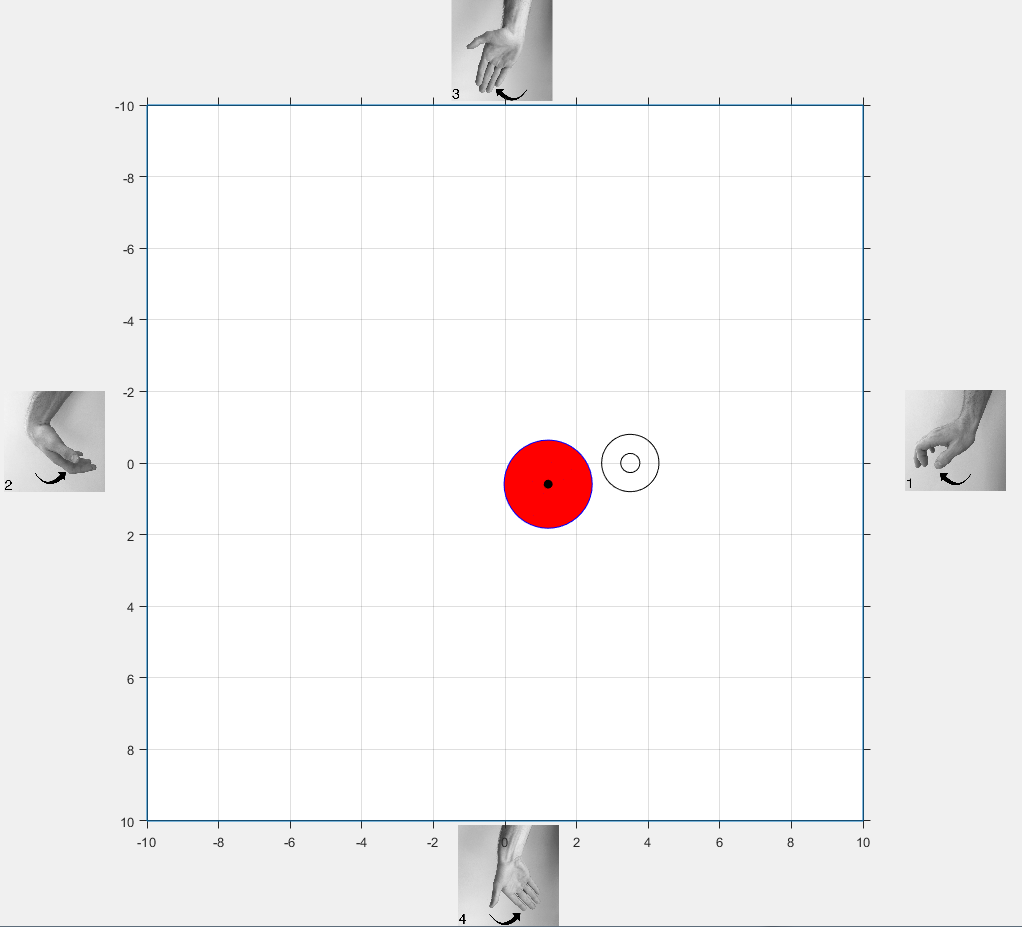
\includegraphics[width=0.4\textwidth]{figures/Paper/perftestGUI}
	\caption{The implemented interface for the modified Fitts' Law test. The user controlled the red cursor with the centred bold mark. The target consisted of a circle with a larger circle surrounding it. The user was instructed in matching the cursor with the target, where the bold mark should be positioned inside the inner circle of the target, and the outer circle of the cursor should be matched in size with the outer circle of the target. The cursor would then turn green to indicate the matching was correct.}
	\label{fig:fittsLawTask}
\end{figure}

Originally the Fitts' Law task had a single performance measure, \textit{throughput} (TP) \cite{Fitts1954}. TP uses the relationship between time taken to reach a certain target in seconds ($MT$) and the index of difficulty (ID), and is defined as:

\begin{equation} \label{eq:TP}
TP=\frac{1}{N}\sum_{i=1}^{N} \frac{ID_i}{MT_i} 
\end{equation}

where $i$ is a specific movement and $N$ is the total number of movements. ID relates to the target's width $W$ and distance $D$ from origin. The ID is calculated as: 

\begin{equation} \label{eq:ID}
ID=log_2(\frac{D}{W}+1)
\end{equation}

According to \cite{Scheme2013a}, it is in practice most resourceful to use a variety of ID's in a Fitts' Law task. Based on this assumption, the target ID's seen in \tabref{tab:P:ID} were calculated for this study.

\begin{table}[H]
	\centering
	\caption{The index of difficulty used in the Fitts' Law task.}
	\label{tab:P:ID}
	\begin{tabular}{l|l|l}
		
		D		 & W	         & ID				   \\ \hline
		28.0     & $\frac{1}{3}$ & 6.41                \\ \hline
		24.5     & $\frac{1}{3}$ & 6.22                \\ \hline
		22.0     & $\frac{1}{3}$ & 6.01                \\ \hline
		18.5     & $\frac{1}{3}$ & 5.82                \\ \hline
		16.0     & $\frac{1}{3}$ & 5.61                \\ \hline
		13.0     & $\frac{1}{3}$ & 5.32                \\ \hline
		12.5     & $\frac{1}{3}$ & 5.27                \\ \hline
		9.5      & $\frac{1}{3}$ & 4.88                \\ \hline
	\end{tabular}
\end{table}

Further performance measures were included similar to previously reported in \cite{Scheme2013, Scheme2013a}. These measures consists of \textit{Path Efficiency}, \textit{Overshoot}, \textit{Stopping Distance} and \textit{Completion Rate}. The additional four measures were added to quantitatively assess performance of naturalness, spontaneity, and compensatory motions during control.  